\documentclass{lni}
\let\ifpdf\relax
\IfFileExists{latin1.sty}{\usepackage{latin1}}{\usepackage{isolatin1}}

\usepackage{graphicx}

%neue Rechtschreibung
\usepackage{ngerman}
\usepackage[colorlinks=false,pdfborder=0 0 0]{hyperref} %URLS
\usepackage[hyphenbreaks]{breakurl}
\usepackage{listings} % XML Listing

\usepackage{acronym}
\usepackage{picins} % Grafiken mit hpic einfuegen
% deutsche Silbentrennung
\usepackage[ngerman]{babel} 
% wegen deutschen Umlauten
\usepackage[ansinew]{inputenc}

\author{
	Tobias Schmid, Andreas Kn�pfle \\ 
	\\ 
	Fachbereich Informatik \\ 
	Freie Universitt Berlin \\ 
	Anschrift \\ 
	Postleitzahl Ort \\ 
	emaiaddresse@autor1 \\
	emaiaddresse@autor2
}
\title{Communities im Co-Author-Graphen}
\begin{document}
\maketitle

\begin{abstract}
Im Rahmen einer Semersterarbeit werden die Metadaten des DBLP-Datensatzes analysiert. Diese Metadaten enthalten Informationen �ber die in der DBLP-Datenbank gespeicherten wissenschaftlichen Publikationen. Auf dieser Grundlage wird ein Co-Author-Graph erzeugt, der die im Datensatz auftretenden Autoren �ber ihre gemeinsamen Publikationen verbindet. Es wird analysiert, ob Gemeinschaften (Communities) unter den Autoren ausgemacht werden k�nnen und welche Rollen die Autoren innerhalb ihrer Gemeinschaften �bernehmen. Abschlie�end wird nach einer geeigneten M�glichkeit gesucht den Co-Author-Graphen und die Ergebnisse der Analyse auf geeignete Weise zu visualisieren.  
\end{abstract}
\newpage
\tableofcontents
\newpage
\section{Einleitung}

Der \acs{DBLP} Datensatz beinhaltet eine gro�e Sammlung wissenschaftlicher Publikationen und deren Meta-Daten aus dem Bereich Informatik. Insgesamt sind bereits mehr als 1,8 Millionen Publikationen aufgenommen worden (\cite{dblp_org}). Aus diesen Daten l�sst sich ein Co-Autor-Graph ableiten, welcher alle Autoren als Knoten und Publikationen zwischen ihnen als gemeinsame Kanten beschreibt. Dieser Graph kann durch graphentheoretische Betrachtungen analysiert werden.\\ 

Anschaulich hei�t das: Haben zwei Autoren miteinander publiziert, sind deren Knoten durch eine Kante verbunden. Das Gewicht einer Kante zeigt zus�tzlich die Anzahl der gemeinsamen Publikationen an.\\

Bei einem Datensatz dieser Gr��e k�nnte eine Analyse dieses Graphen repr�sentative Aussagen �ber die Autoren und deren Umfeld geben. 
Somit wird die wissenschaftliche Fragestellung dieser Arbeit wie folgt festgelegt: \\\\

 Welche Charaktereigenschaften weisen die Autoren und ihr Umfeld im Co-Autorgraph der DBLP auf? \\\\

% { Methoden }
Um dieser Frage nachzukommen, wird eine Infrastruktur entwickelt, die es erm�glicht den Co-Autor-Graphen zu generieren und zu visualisieren. Zus�tzlich m�ssen Werkzeuge entwickelt werden, die es erlauben den Graphen zu analysieren. 

% {Motivation}
% {Hauptfrage: Welche Charaktereigenschaften weisen die Autoren und ihr Umfeld im Co-Autorgraph der DBLP auf?}


\section{Ausgangssituation}

Als Datenquelle f�r den Co-Autor-Graphen werden die Metadaten der \acs{DBLP}-Datenbank im \acs{XML}-Format benutzt \cite{dblp_xml}.
Die Metadaten bestehen aus einer Liste der wissenschaftlichen Artikel mit Titel, Datum, Autoren und zus�tzlichen Informationen �ber die Ver�ffentlichung. \\

In \ref{listing:xml_source} ist ein Ausschnitt aus dieser \acs{XML} Quelle abgebildet. Aus dieser Quelle kann der Co-Autor-Graph erzeugt werden, da jeder Artikel alle beteiligten Autoren enth�lt und somit auf Knoten und Kanten im Graphen abgebildet werden kann.


%\subsubsection{Die DBLP Daten}


\section{Randbedingungen}

Um den Co-Autor-Graphen zu analysieren, wird eine effiziente Form des Datenzugriffs ben�tigt. Um diesen Zugriff technisch umzusetzen wird im Weiteren die Graphdatenbank Neo4J verwendet. Mit Hilfe von Neo4J kann der Graph einfach und effizient gespeichert und traversiert werden. Zus�tzlich k�nnen Meta-Informationen zu den Knoten und Kanten in der Datenbank verwaltet werden, womit diese durch Analyseergebnisse angereichert werden k�nnen. Weiterhin unterst�tzt Neo4J die Entwicklung von Algorithmen auf Graphen und bietet bereits einige Implementierungen dieser.\\


%\subsubsection{Neo4J Datenbank}

%\subsubsection{Neo4J Datenbank}


\section{Communities im Co-Autor-Graphen}


Die Autoren sind durch gemeinsame Publikationen im Co-Autor-Graphen miteinander verbunden. Viele Publikationen zwischen zwei Autoren lassen auf eine starke Verbindung zwischen diesen schlie�en. Durch diese Verbindungen k�nnen sich Gemeinschaften unter den Autoren bilden.\\

% {Teilfrage: Lassen sich Gemeinschaften/Communities in den dblp Daten finden?}
Im Folgenden wird also untersucht, ob im Co-Autor-Graphen der DBLP Gemeinschaften unter den Autoren zu finden sind. \\
Sollten Gemeinschaften gefunden werden k�nnen, ergeben sich die weiteren Fragestellungen: \\\\

Wie stark unterscheiden sich die Communities in ihrer Gr��e ? \\
Wie lassen sich die Communities noch anders charakterisieren (nicht nach der Gr��e) ? \\
Ist ein Zusammenhang zwischen Gr��e und Charakter einer Community erkennbar ? \\\\

% { Methoden }
%Community-Algorithmus
Um diese Gemeinschaften, weiterhin mit dem englischen Begriff Communities bezeichnet, finden zu k�nnen, wird der in \cite{communityDetection} beschriebene Community-Detection Algorithmus eingesetzt. Dieser Algorithmus findet Communities und deren Zusammensetzung als Hierarchiestruktur. Die Ergebnisse des Community-Detection Algorithmus werden in der Neo4J Datenbank gespeichert. \\

Die oberste ebene der Hierarchiestruktur, die die Zusammensetzung der Communities beschreibt, besteht aus den gefundenen Communities (Top-Level-Communities). Jede dieser Communities besteht wieder aus kleineren Communities und diese wieder aus Communities usw.. So gibt es mehrere Stufen, wobei die unterste Ebene die Autoren darstellt. \\

%Gr��e der Community
Die Gr��e jeder Top-Level-Community und ihrer Untergruppen kann durch einen rekursiven Algorithmus berechnet werden. \\

%Conductance einer Community
Die Conductance einer Community zeigt das Verh�ltnis der Anzahl der Kanten, welche diese Community mit einer anderen verbindet, zu der Anzahl der Kanten innerhalb der Community an. Dies kann als zus�tzliche Charakterisierung verwendet werden. \\


% Mit Mit Gr��e und Conductance k�nnen die Communities charakterisiert werden.

% { Ergebnisse }

\subsection{Der Community Algorithmus}

TODO ...

\subsection{Die Messungen}

Im Folgenden werden die Messungen n�her beschrieben. Dabei wird zuerst auf die Messung der Community Gr��en und danach auf die Messung der Conductance eingegangen.

	\subsection{Gr��e}
	
	Da die Communities Hierarchisch aufgebaut sind, k�nnen die Gr��en der Communities auf den verschiedenen Hierarchie-Ebenen gemessen werden. Dazu sollte die Gr��e der unterste Ebene (eine ebene �ber der Autor Ebene) gleich der Anzahl der Autoren sein, welche direkt mit dieser Community verbunden sind. Die Gr��e jeder Community in einer h�heren Ebene setzt sich dann durch die Anzahl der beinhaltenden Autoren der Unterebenen zusammen. So kann f�r alle Communities auf allen Ebenen die genaue Gr��e bestimmt werden. \\
	
	Um diese Gr��en f�r den Co-Author-Graphen zu bestimmen, wird ein rekursiever Algorithmus entwickelt, welcher auf den einzelnen Ebenen f�r die Communities die Gr��en berechnet. In folgendem Pseudocode-Listing ist der rekursive Algorithmus abgebildet.
	
	\begin{verbatim}

	HashMap<Long, Object> counts;	
	
	long count(Node community)
	-- Wenn Community Untercommunities hat	
	---- long counter_community
	---- F�r jede Untercommunity in Community
	------ long count = count(Untercommunity)
	------ counter_community += count
	---- counts.put(community.getId(), counter_community)
	---- return counter_community
	--Sonst
	---- return 1
	
	\end{verbatim}
	
	Der Algorithmus startet bei dem ersten Community Knoten welcher der Methode �bergeben wird. Es werden alle \textit{BELONGS\_TO} Beziehungen verwendet, um alle Unter-Communities des Community Knotens zu finden. dann wird der Algorithmus rekursiv auf alle Unter-Communities angewandt. Wenn der Algorithmus bei einem Autor Knoten angekommen ist, wird f�r diesen Autor Knoten der Wert eins zur�ckgegeben und schlussendlich die entsprechenden Anzahlen der Communities in der Rekursion nach oben durchgegeben. Die Anzahl an Autoren in einer Community wird  jeweils gespeichert, um diese Werte in die Datenbank schreiben zu k�nnen.


	\subsection{Conductance}
	
	Die Conductance einer Community ist durch folgende Formel \cite{conductance_formel} bestimmt: \\\\
	
		$ \frac{c(C,G \backslash C)}{min(k_{C},k_{G \backslash  C})} $ \\\\
		
	Dabei haben die Werte die folgende Bedeutung:
	
	\begin{itemize}
	
	\item C: Community
	\item G: Gesamtgraph
	\item c(C, G \textbackslash C): Cut size von C
	\item $ k_{C} $: Anzahl Kanten von C
	\item $ k_{G \backslash C} $: Anzahl Kanten von G ohne C

	\end{itemize}
		
	Somit ist die Conductance ein Verh�ltnis der Publikations-Kanten ,welche aus der Community heraus gehen zu der Anzahl an Publikations-Kanten innerhalb der Community. \\
	
	Der erwartete Wertebereich der Conductance liegt zwischen Null und Eins. Dabei w�rde Null bedeuten, dass keine Kanten nach au�en gehen und die Community komplett isoliert ist. Ein Wert gr��er Eins w�rde bedeuten, dass die Community mehr Kanten nach au�en hat, als innere Kanten. Da der Community Algorithmus zur Erkennung von Communities die Anzahl der Kanten zwischen den Knoten betrachtet, ist es eher unwahrscheinlich, dass eine Community mit einer Conductance gr��er Eins entsteht.



	\subsection{Ergebnisse in die Datenbank schreiben}

	Da sehr viele Knoten und Kanten in der Datenbank gespeichert sind und alle Messergebnisse zu den jeweiligen Knoten und Kanten in die Datenbank geschrieben werden sollen, wird eine effektive M�glichkeit ben�tigt die gro�e Menge an Messergebnissen in die Datenbank zu schreiben.
	

\subsection{Ergebnisse der Messungen}

	\subsection{Gr��e}

	\subsection{Conductance}

\subsection{ Analyse der Ergebnisse }

% { Diskussion }


% {Teilfrage: Sind verschieden Rollenverteilungen unter den Autoren einer Community erkennbar ?}
% { Methoden }

% { Ergebnisse }

% { Diskussion }
\section{Visualisierung des Co-Autor-Graphen}
Um Informationen �ber einzelne Autoren und deren Communities aus dem Co-Autor-Graphen gewinnen zu k�nnen muss der Co-Author-Graph auf geeignete Art visualisiert werden. Daher wird versucht folgende Frage zu beantworten: 

 \begin{center}
\textit{L�sst sich das Umfeld eines Autors im Co-Autor-Graphen und seine Community visualisieren?}
\end{center}
 Der in der Neo4j-Datenbank gespeicherte Graph kann zwar �ber die in Neo4j eingebauten Bordmittel bereits teilweise visualisiert werden, allerdings funktioniert die Visualisierung bei dieser Datenmenge nur stark eingeschr�nkt. Vor allem die Tatsache, dass bei dieser Art von Visualisierung der jeweils betrachtete Teil des Graphen dynamisch aus der Datenbank gelesen werden muss, schr�nkt den Gesamtprozess stark ein. \\
 Daher wird mit einem neuen Modul f�r die in Abschnitt \ref{randbendingingen} beschriebene Applikation der gesamte Graph mit allen enthaltenen Knoten in eine statische \acs{HTML}-Struktur exportiert. 
 \subsection{Visualisierung des Graphen mit \acs{HTML}}
  Abbildung \ref{img:web} zeigt eine der durch die vorher beschriebe Methode entstandenen \acs{HTML}-Seiten. Die einzelnen Autoren untereinander enthalten \acs{HTML}-Verlinkungen zu allen Nachbarautoren und der Communities (pro jede Hierarchieebene eine) denen sie angeh�ren. 
 \begin{center}
					\hpic{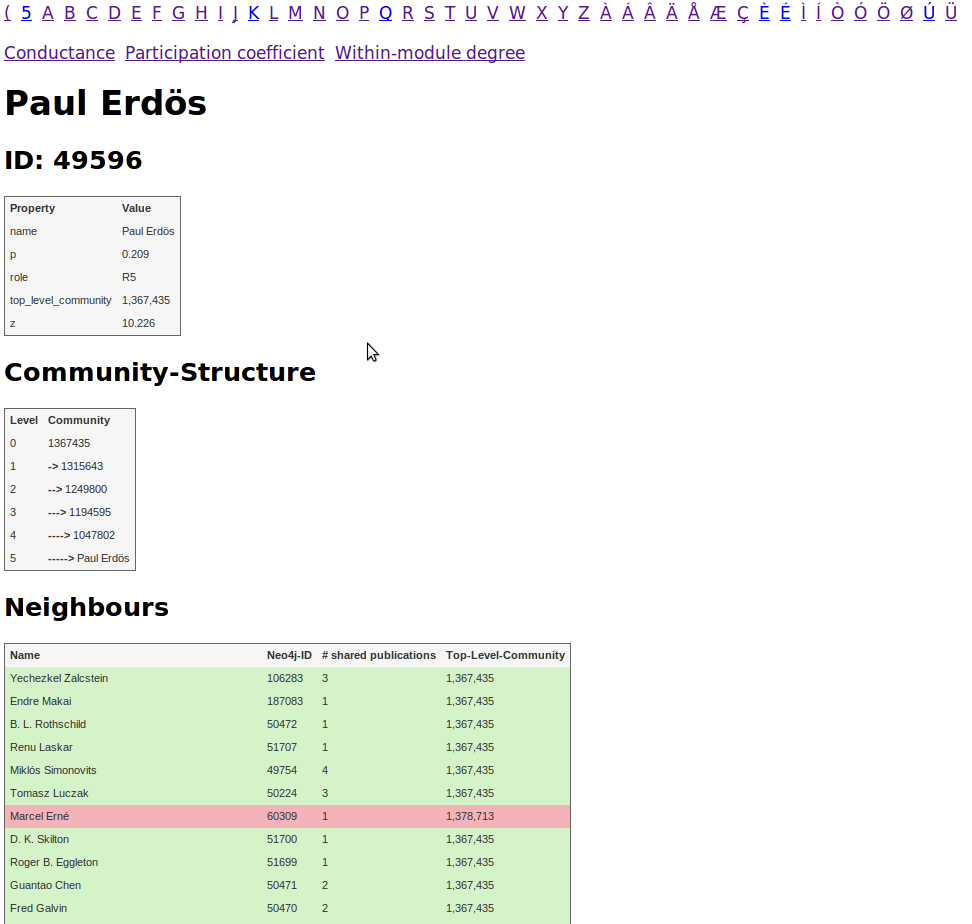
\includegraphics[width=1\textwidth]{images/web}
					} \newcaption{HTML-Darstellung vom Autorknoten Paul Erd�s}
					\label{img:web}
	\end{center}
  Diese Art der Visualisierung verhindert, dass der Graph bei Betrachtung dynamisch aus der Datenbank geladen werden muss, da dies bereits zum Zeitpunkt des \acs{HTML}-Exports geschieht. Auf diese Art kann das Umfeld eines Autors effizient und schnell durchsucht werden. Durch einen alphabetischen Index k�nnen Autoren schnell gefunden und analysiert werden. 
% { Methoden }

% { Ergebnisse }

% { Diskussion }


\section{Schluss}


% { Ergebnisse }

% { Diskussion }

% Weiterentwicklung

Durch eine modulare Architektur, ist es einfach neue Messmodule in das System zu integrieren und Ergebnisse in die Datenbank zu schreiben. Dadurch ist die Infrastruktur beliebig erweiterbar. Es k�nnten neue Messwerte wie beispielsweise die \textit{Significance} (Stabilit�t einer Community) eingef�hrt werden, um noch mehr �ber die Daten aussagen zu k�nnen. Auch w�re eine Betrachtung der zeitlichen Entwicklung von Communities und Autoren m�glich.\\

Weiterhin w�re es m�glich neue Parser zu entwickeln, um die Messungen auch auf andere Daten durchzuf�hren. 



\section*{Abk�rzungsverzeichnis} 
\addcontentsline{toc}{section}{Abk�rzungsverzeichnis}

		\begin{acronym}
		 	\acro{DBLP}{DataBase systems and Logic Programming}
		 	\acro{XML}{Extensible Markup Language}
		 	
		\end{acronym}


\nocite{dblp_org}
\nocite{dblp_xml}
\nocite{conductance_formel}

\bibliographystyle{alphadin}
\bibliography{dblp_communities}

\end{document}
